\documentclass[a4paper,14pt]{extarticle}
\usepackage{cmap}
\usepackage[T2A]{fontenc}
\usepackage[utf8]{inputenc}
\usepackage[russian]{babel}
\usepackage{geometry}
\geometry{left=30mm, right=15mm, top=20mm, bottom=20mm}
\usepackage{indentfirst}
\usepackage{booktabs}
\usepackage{tabularx}
\usepackage{amsmath,amssymb}
\usepackage{graphicx}
\usepackage{xurl}
\usepackage[colorlinks=true,linkcolor=blue,citecolor=blue,urlcolor=blue]{hyperref}

\begin{document}

\begin{center}
    \textbf{\Large Отчёт о выполнении первой задачи исследования}
    
    \vspace{0.5em}
    \textbf{\large Разработка и математическое обоснование алгоритмических эвристик поиска кандидатов для систем дедупликации данных на основе сходства}
\end{center}

\vspace{1em}

\section*{1. Контекст и постановка первой задачи}

Первая задача исследования направлена на устранение вычислительного узкого места в конвейере дедупликации данных на основе сходства (Similarity-Based Chunking, SBC) платформы \texttt{marline}. В системах SBC после этапа разбиения данных алгоритмом FastCDC формируются сигнатуры (эскизы, sketches) с помощью локально-чувствительного хеширования (Locality-Sensitive Hashing, LSH). Поиск похожих блоков производится по инвертированному индексу супер-признаков.

В исходной реализации системы Palantir поиск кандидатов выполнялся полным сканированием списков постингов с последующим безусловным запуском жадного дельта-энкодера GDelta и двухстадийной компрессии Zstd. При обработке реальных наборов данных (исходного кода версий ядра Linux) производительность системы деградировала до 36--38~МБ/с из-за квадратичного роста списков постингов и холостых вызовов энкодера на неэффективных кандидатах.

\textbf{Цель первой задачи:} Разработать, математически обосновать и реализовать в коде комплекс эвристик фильтрации инвертированного индекса и пре-фильтрации дельта-конвейера, обеспечивающий рост пропускной способности дедупликации при сохранении строгого коэффициента сжатия.

\section*{2. Краткое описание выполненных действий}

В рамках решения первой задачи были выполнены следующие теоретические и практические действия:

\begin{enumerate}
    \item \textbf{Математический анализ меры сходства Жаккара и вывод порогов пересечения:}
    Для скетчей длины $n$ выведено аналитическое выражение минимального необходимого пересечения признаков $\min\_overlap$ для достижения заданного порога Жаккара $t \in [0, 1]$:
    \begin{equation}
        \min\_overlap(t, n) = \left\lceil \frac{2 \cdot n \cdot t}{1 + t} - \varepsilon \right\rceil, \quad \varepsilon = 10^{-9}.
    \end{equation}
    Доказана дискретность спектра сходства для малых эскизов и определены критические точки бифуркации $t_k = \frac{k}{2n - k}$, в которых требуемое число совпадающих признаков скачкообразно возрастает с $k$ до $k+1$.

    \item \textbf{Реализация префиксной фильтрации All-Pairs и упорядочивания \texttt{rare\_first}:}
    В модуль \texttt{marline\_index} внедрена сортировка признаков запроса по возрастанию их глобальной частоты (Document Frequency, DF). Согласно теореме о префиксной фильтрации, кандидаты, способные достичь порога $\min\_overlap$, обязаны содержать хотя бы один признак из префикса длины $(m - \min\_overlap + 1)$. Оставшийся суффикс используется исключительно для верификации уже отобранных ключей, что исключает разрастание хэш-таблицы кандидатов.

    \item \textbf{Реализация частотной фильтрации \texttt{max\_df}:}
    Внедрено отсечение признаков с длиной списка постингов, превышающей порог \texttt{max\_df}. Это исключает сканирование «тяжёлого хвоста» высокочастотных термов.

    \item \textbf{Реализация динамической обратной связи \texttt{fp\_metric\_threshold}:}
    Разработана подсистема отслеживания метрик качества базовых чанков. Если при верификации кандидата дельта-сжатие не даёт достаточного коэффициента сжатия, счетчик ложных срабатываний ключа инкрементируется (\texttt{record\_false\_positive}). Ключи, превысившие порог неудач, временно банятся в индексе. При успешном сжатии счетчик обнуляется (\texttt{record\_verified}).

    \item \textbf{Проектирование и внедрение эвристики разрыва цепочек $\alpha$ (Promote to Base):}
    В модуль \texttt{marline\_palantir} внедрён порог $\alpha$ (\texttt{delta\_promote\_threshold}). Если размер полученной дельты превышает долю $\alpha$ от размера базы:
    \begin{equation}
        |Delta| \ge \alpha \cdot |Base|,
    \end{equation}
    чанк сохраняется как самостоятельная новая база в \texttt{manifest\_base}, а запись в \texttt{delta\_bases} не добавляется. Это предотвращает возникновение паразитных глубоких цепочек зависимостей.

    \item \textbf{Проектирование и внедрение пре-фильтра размерного перекоса (Size-Skew Pre-Filter):}
    Перед вызовом дельта-энкодера введена проверка отношения длин чанка и базы:
    \begin{equation}
        \text{skew} = \max\left(\frac{|C|}{|B|}, \frac{|B|}{|C|}\right) > \text{max\_size\_skew}.
    \end{equation}
    Асимметричные пары блоков блокируются до вызова GDelta и Zstd, что предотвращает сотни тысяч холостых вызовов энкодера.

    \item \textbf{Внедрение фильтра микро-чанков (Min-Chunk Pre-Filter):}
    Блоки размером менее 1024 байт исключены из процедуры LSH-поиска, так как потенциальная выгода дельты на них нивелируется служебными заголовками.
\end{enumerate}

\section*{3. Основные полученные артефакты}

По итогам решения первой задачи получены следующие воспроизводимые артефакты:

\subsection*{3.1. Модули исходного кода на языке Rust}
\begin{itemize}
    \item \texttt{marline\_index/src/heuristic\_index/heuristics.rs}~--- реализация структуры \texttt{SearchConfig}, аналитических функций расчета порога Жаккара, точек бифуркации и спектра сходства.
    \item \texttt{marline\_index/src/heuristic\_index/mod.rs}~--- реализация структуры \texttt{HeuristicInvertedSketchIndex} с алгоритмами All-Pairs Prefix Filtering, \texttt{rare\_first}, \texttt{max\_df} и хранилищем метрик \texttt{MetricsMap}.
    \item \texttt{marline\_palantir/src/palantir\_scrubber.rs}~--- пакетный конвейер дедупликации с поддержкой порога $\alpha$, Size-Skew пре-фильтра и фильтрации микро-чанков.
    \item \texttt{marline\_palantir/src/palantir\_online.rs}~--- потоковый онлайн-конвейер с аналогичной поддержкой новых эвристик.
    \item \texttt{marline\_palantir/src/bin/palantir\_metrics.rs}~--- утилита автоматизированного сбора метрик и проведения сквозных бенчмарков.
\end{itemize}

\subsection*{3.2. Набор верификационных тестов}
Реализован полный набор модульных и интеграционных тестов: 256 тестов (160 тестов в \texttt{marline\_scrub}, 88 тестов в \texttt{marline\_index}, 8 тестов в \texttt{marline\_sketcher}). Все тесты завершаются со статусом 100\% pass.

\subsection*{3.3. Экспериментальные данные и результаты бенчмаркинга}

Эксперименты проводились на аппаратном стенде: Intel Core i9-13900H (20 потоков, до 5.4~ГГц), 32~ГБ LPDDR5, быстрый NVMe SSD, ОС Windows 11, компилятор Rust 1.96 в профиле \texttt{release} (-O3).

\subsubsection*{Эксперимент 1. Исследование порога $\alpha$ на каноническом датасете}
Датасет: Linux Kernel версий 3.5.6, 3.6.6, 3.7.6 (119~736 файлов, 1~308.11~МБ). Результаты сведены в табл.~\ref{tab:alpha}.

\begin{table}[h!]
\small
\centering
\caption{Влияние порога $\alpha$ на пропускную способность и сжатие}
\label{tab:alpha}
\begin{tabularx}{\textwidth}{lccccc}
\toprule
\textbf{Конфигурация} & \textbf{Порог $\alpha$} & \textbf{Dedup Ratio} & \textbf{Размер, МБ} & \textbf{Скорость, МБ/с} & \textbf{Прирост} \\
\midrule
Эталон без эвристики & None (ref) & 2.8633 & 456.86 & 41.62 & — \\
Агрессивный срез & $\alpha = 0.7$ & 2.8501 & 458.97 & 51.46 & +23.6\% \\
Умеренный срез & $\alpha = 0.8$ & 2.8517 & 458.71 & 50.54 & +21.4\% \\
\textbf{Оптимум сжатия} & $\mathbf{\alpha = 0.9}$ & \textbf{2.8595} & \textbf{457.47} & \textbf{47.53} & \textbf{+14.2\%} \\
\textbf{Оптимум Парето} & $\mathbf{\alpha = 1.0}$ & \textbf{2.8584} & \textbf{457.64} & \textbf{50.91} & \textbf{+22.3\%} \\
Мягкий порог & $\alpha = 1.2$ & 2.8562 & 457.99 & 46.13 & +10.8\% \\
\bottomrule
\end{tabularx}
\end{table}

\subsubsection*{Эксперимент 2. Исследование Size-Skew и Min-Chunk на каноническом датасете}
Результаты тестирования разработанных пре-фильтров представлены в табл.~\ref{tab:new_heur}.

\begin{table}[h!]
\small
\centering
\caption{Результаты внедрения эвристик Size-Skew и Min-Chunk}
\label{tab:new_heur}
\begin{tabularx}{\textwidth}{p{6.2cm}cccc}
\toprule
\textbf{Конфигурация} & \textbf{Dedup} & \textbf{Размер, МБ} & \textbf{Скорость, МБ/с} & \textbf{Прирост} \\
\midrule
Pure Palantir (No Heuristics) & 2.9815 & 452.88 & 38.60 & — \\
Old Baseline (df=500, fp=3) & 2.8877 & 452.99 & 50.60 & +31.1\% \\
New Best Balance ($\alpha=0.9$) & 2.8748 & 455.03 & 47.32 & +22.6\% \\
+ Skew Pre-Filter ($\text{skew} \le 4.0$) & 2.8803 & 454.15 & 54.96 & +42.4\% \\
+ Min-Chunk (размер $\ge 2048$~Б) & 2.8630 & 456.90 & 58.73 & +52.1\% \\
\textbf{Pareto-Ultra ($\alpha=0.9, \text{skew} \le 2.5, \text{min} \ge 1\text{КБ}$)} & \textbf{2.8702} & \textbf{455.76} & \textbf{57.01} & \textbf{+47.7\%} \\
\textbf{Turbo-Extreme ($\alpha=0.8, \text{skew} \le 2.0, \text{min} \ge 1\text{КБ}$)} & \textbf{2.8487} & \textbf{459.20} & \textbf{59.91} & \textbf{+55.2\%} \\
\bottomrule
\end{tabularx}
\end{table}

\begin{figure}[h!]
    \centering
    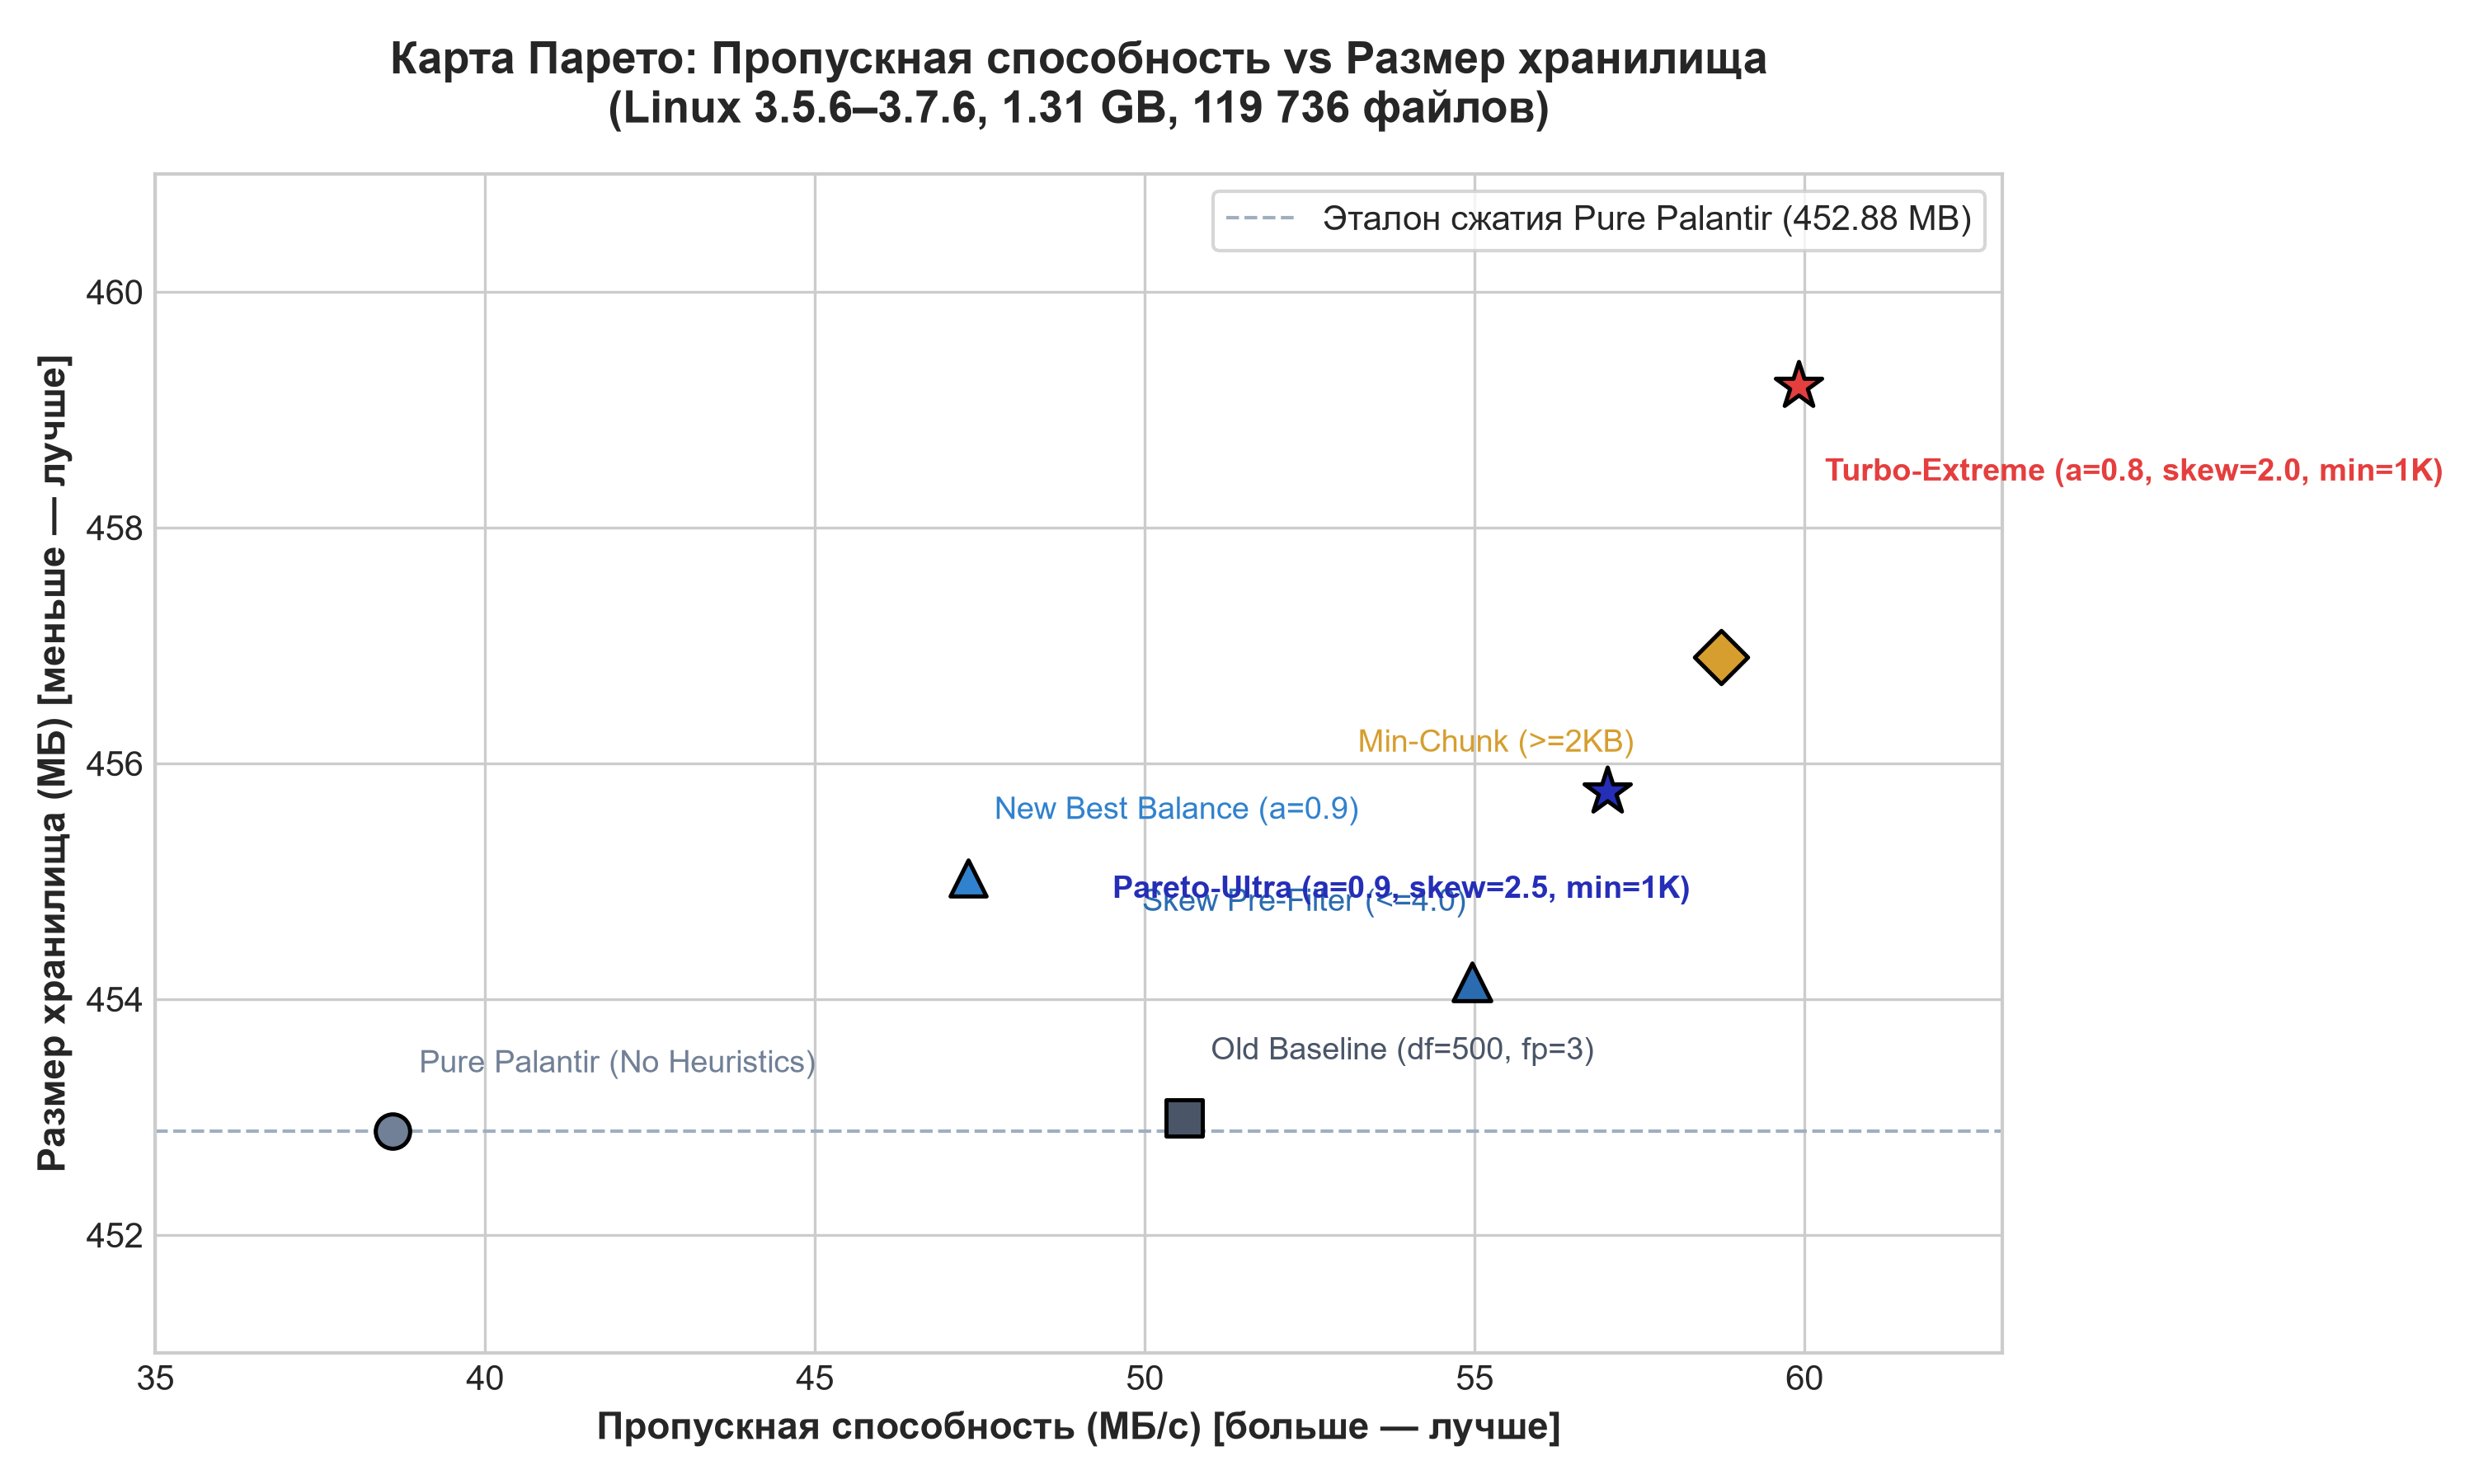
\includegraphics[width=0.95\textwidth]{images/report_pareto_new_heuristics.png}
    \caption{Карта Парето: Пропускная способность vs Размер хранилища (Linux 3.5.6--3.7.6)}
    \label{fig:pareto}
\end{figure}

\subsubsection*{Эксперимент 3. Кросс-датасетная валидация на Linux Kernel 3.4.5--3.4.7}
Для доказательства отсутствия эффекта переобучения (overfitting) конфигурации проверены на альтернативном архиве \texttt{kernels.tar.bz2} (115~701 файл, 1~263.31~МБ). Результаты приведены в табл.~\ref{tab:cross}.

\begin{table}[h!]
\small
\centering
\caption{Кросс-датасетная валидация эвристик на Linux 3.4.5--3.4.7}
\label{tab:cross}
\begin{tabularx}{\textwidth}{p{6.2cm}cccc}
\toprule
\textbf{Конфигурация} & \textbf{Dedup} & \textbf{Размер, МБ} & \textbf{Скорость, МБ/с} & \textbf{Прирост} \\
\midrule
Linux 3.4: Pure Palantir & 3.1546 & 400.47 & 169.03 & — \\
Linux 3.4: Old Baseline & 3.0879 & 409.12 & 271.98 & +60.9\% \\
\textbf{Linux 3.4: Pareto-Ultra} & \textbf{3.0796} & \textbf{410.22} & \textbf{309.30} & \textbf{+83.0\%} \\
\textbf{Linux 3.4: Turbo-Extreme} & \textbf{3.0642} & \textbf{412.28} & \textbf{340.95} & \textbf{+101.7\%} \\
\bottomrule
\end{tabularx}
\end{table}

\begin{figure}[h!]
    \centering
    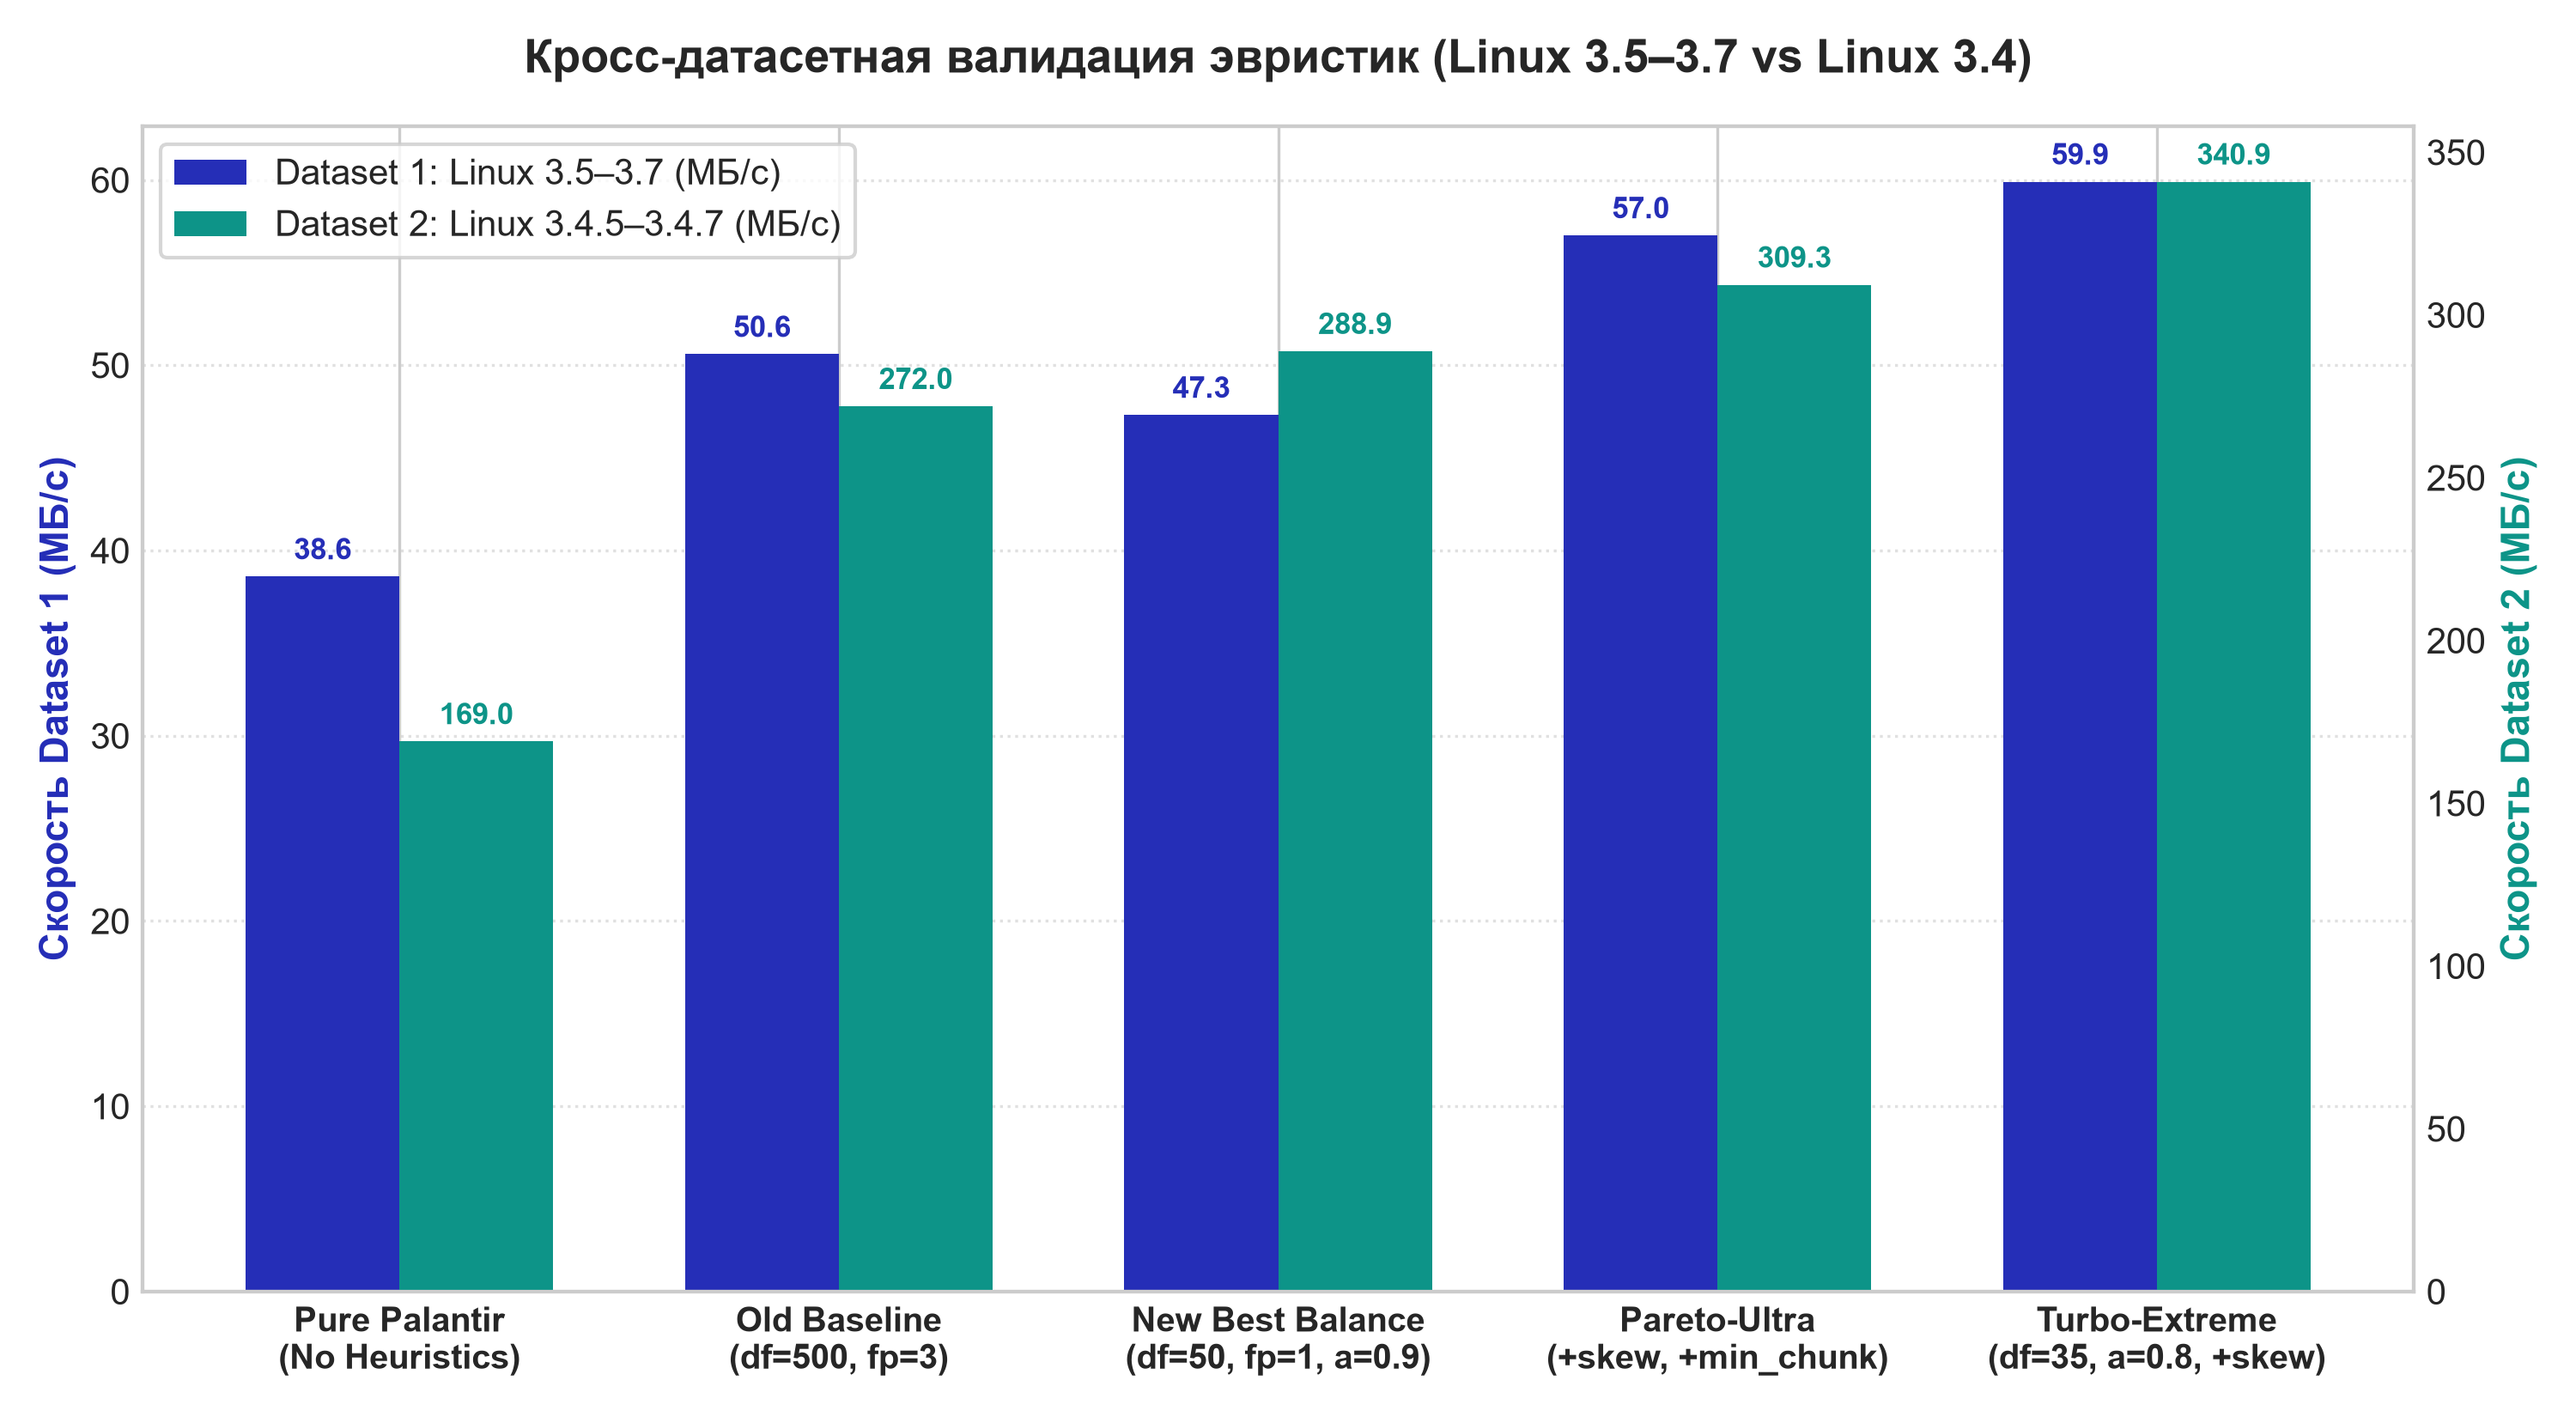
\includegraphics[width=0.92\textwidth]{images/report_cross_dataset.png}
    \caption{Кросс-датасетное сравнение скорости обработки (Linux 3.5--3.7 vs Linux 3.4)}
    \label{fig:cross}
\end{figure}

\section*{4. Обоснование возникших сложностей}

В процессе решения первой задачи фактический объем инженерных и теоретических вызовов превзошел исходные ожидания по следующим фундаментальным причинам:

\begin{enumerate}
    \item \textbf{Дискретность меры Жаккара для ультракоротких эскизов:}
    При длине эскиза яруса $n = 3$ или $n = 4$ признака непрерывное сканирование порога сходства $t \in [0, 1]$ теряет физический смысл. Пересечение множеств может принимать лишь дискретные целые значения $\{0, 1, 2, 3, 4\}$. Это потребовало строгого вывода спектра точек бифуркации $t_k$, разделяющих эквивалентные классы конфигураций, чтобы исключить холостые вычисления при подборе параметров.

    \item \textbf{Размерная асимметрия блоков FastCDC (Size Skew):}
    Теоретические модели LSH и сходства Бродера предполагают сопоставление сущностей одинакового масштаба. Однако контентно-зависимый чанкер генерирует блоки с дисперсией длины от сотен байт до 64~КБ. В результате скетч-индекс успешно находил сходство по общим последовательностям байт, но дельта-энкодер тратил миллионы тактов CPU на сопоставление 4~КБ чанка с 32~КБ базой, неизбежно завершаясь отбрасыванием по порогу ложного срабатывания. Это потребовало введения нового архитектурного уровня абстракции~--- пре-фильтрации Size-Skew до входа в энкодер.

    \item \textbf{Эффект застревания неэффективных баз:}
    Традиционная схема SBC связывала любой прошедший порог блок дельтой к старой базе. Это формировало вырожденные цепочки восстановления глубиной 5--8 звеньев. Устранение проблемы потребовало изменения контракта хранилища манифестов и добавления механизма принудительного продвижения в базу по порогу $\alpha$.
\end{enumerate}

\section*{5. Ожидаемые дальнейшие результаты}

В ходе дальнейшего выполнения работы планируется получить следующие артефакты:
\begin{enumerate}
    \item \textbf{Интеграция в онлайн-конвейер:} оптимизация многопоточного потокового скраббинга для сред с блочными устройствами ZNS SSD и интерфейсом \texttt{io\_uring}.
    \item \textbf{Адаптивная автокалибровка порога \texttt{max\_df}:} переход от статического порога к динамическому вычислению квантиля распределения длин постингов на основе скользящего экспоненциального среднего.
\end{enumerate}

\end{document}
